\begin{figure}
    \centering
    \caption{Forças internas: seção em um sólido qualquer}
    \begin{subfigure}[b]{0.3\textwidth}
        \centering
        \begin{tikzpicture}[scale=0.6]
            \draw [->] (0,0,0) -- (4,0,0) node[anchor = west] {$z$};
            \draw [->] (0,0,0) -- (0,8,0) node[anchor = south] {$x$};
            \draw [->] (0,0,0) -- (0,0,4) node[anchor = east] {$y$};
        \end{tikzpicture}
        \caption{$y=x$}
        \label{fig:y equals x}
    \end{subfigure}
    \hfill
    \begin{subfigure}[b]{0.3\textwidth}
        \centering
        \begin{tikzpicture}[scale=0.6]
            \draw [->] (0,0,0) -- (4,0,0) node[anchor = west] {$x$};
            \draw [->] (0,0,0) -- (0,8,0) node[anchor = south] {$y$};
            \draw [->] (0,0,0) -- (0,0,4) node[anchor = east] {$z$};
            \shade[ball color = blue!60, opacity = 1] (0,4) circle (3cm);
            \draw[green] (-3,4) arc (180:360:3 and 0.6);
            \draw[dashed, green] (3,4) arc (0:180:-3 and 0.6);
            \begin{scope}[canvas is xz plane at y=4]
                \draw (-3,0) arc (0:360:-3); 
            \end{scope}
        \end{tikzpicture}
        \caption{$y=3\sin x$}
        \label{fig:three sin x}
    \end{subfigure}
    \hfill
    \begin{subfigure}[b]{0.3\textwidth}
        \centering
        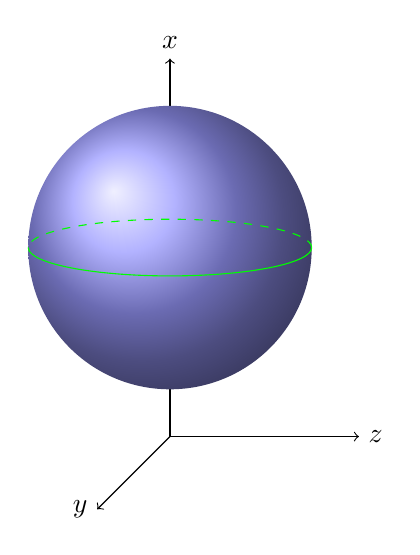
\begin{tikzpicture}[scale=0.6]
            \draw [->] (0,0,0) -- (4,0,0) node[anchor = west] {$z$};
            \draw [->] (0,0,0) -- (0,8,0) node[anchor = south] {$x$};
            \draw [->] (0,0,0) -- (0,0,4) node[anchor = east] {$y$};
            \shade[ball color = blue!40, opacity = 1] (0,4) circle (3cm);
            \draw[green] (-3,4) arc (180:360:3 and 0.6);
            \draw[dashed, green] (3,4) arc (0:180:3 and 0.6);
        \end{tikzpicture}
        \caption{$y=5/x$}
        \label{fig:five over x}
    \end{subfigure}
       \label{fig:forcas_internas}
\end{figure}